\documentclass{article}
\usepackage{amsmath}
\usepackage{amssymb}
\usepackage[a4paper, top=25mm, bottom=25mm, left=25mm, right=25mm]{geometry}
\usepackage{pgfplots}
\usepackage{tikz}
\usepackage{mathtools}
\pgfplotsset{compat=1.18}
\pgfplotsset{compat=newest}
\usepgfplotslibrary{polar}
\usepgfplotslibrary{fillbetween}
\usepgfplotslibrary{patchplots}

\begin{document}
\pagestyle{empty}
\large

\begin{center}
2022-2023 Spring \\MAT124 Final\\(12/06/2023)
\end{center}

\noindent 1. Find the absolute extrema of $f(x,y) = 2x^2-y^2$ on the closed, bounded set $x^2+y^2\leq1$ in the plane.

\hfill

\noindent 2. Sketch the region corresponding to the double integral

\begin{equation*}\int_{-3}^2\int_{x^2}^{6-x}dy\,dx\end{equation*}

\hfill

\noindent and evaluate the integral by writing the equivalent integral with the order of integration reversed.

\hfill

\noindent 3. Using a double integral, find the area enclosed by the upper half of the cardioid $r=1+\sin\theta$.

\hfill

\noindent 4. Sketch the region $R$ bounded above by the elliptic paraboloid $z=2-x^2-y^2$ and below by the paraboloid $z=x^2+y^2$. Using a double integral find the volume of $R$.

\hfill

\noindent 5. Find the surface area of the portion of the sphere $x^2+y^2+z^2=4$ that is above the $xy$-plane and within the cylinder $x^2+y^2=1$.

\hfill

\noindent 6.

\hfill

\noindent (i) Sketch the graph of the region $R$ bounded above by the paraboloid $z=4-x^2-y^2$ and below by the plane $z=4-2x$.

\hfill

\noindent (ii) Evaluate the volume of $R$.

\newpage

\begin{center}
2022-2023 Spring Final (12/06/2023) Solutions\\
(Last update: 7/31/25 (31st of July) 7:34 PM)
\end{center}

\noindent 1) Let $g(x,y,z)=x^2+y^2-1$ and then solve the system of equations below using the method of Lagrange multipliers.

\[
\left.
\begin{array}{ll}
\displaystyle\nabla f =\lambda \nabla g \\
\displaystyle g(x,y) = 0
\end{array}
\right\}\quad
\begin{array}{ll}
\nabla f=\left\langle4x,-2y\right\rangle = \lambda\left\langle2x,2y\right\rangle = \lambda\nabla g \\[0.1cm] x^2+y^2-1=0
\end{array}
\]

\[4x=\lambda(2x)\implies2x(2-\lambda)=0\implies\lambda=2\:\text{or}\:x=0\]
\[-2y=\lambda(2y)\implies-2y(1+\lambda)=0\implies\lambda=-1\:\text{or}\:y=0\]

\hfill

\noindent Now, use the constraint to find the coordinates.

\[\lambda=2\implies y=0\implies x^2+0^2-1=0\implies x=\pm1\]
\[\lambda=-1\implies x=0\implies 0^2+y^2-1=0\implies y=\pm1\]

\hfill

\noindent Evaluate $f$ at these points: $(0,1)$, $(0,-1)$, $(1,0)$, or $(-1,0)$.

\[f(0,1)=2\cdot0^2-1^2=-1,\quad f(0,-1) =2\cdot0^2-(-1)^2=-1,\]
\[f(1,0)=2\cdot1^2-0^2=2,\quad f(-1,0)=2\cdot(-1)^2-0^2=2\]

\hfill

\noindent The \textit{only} critical point occurs at $(0,0)$.

\[\frac{\partial f}{\partial x}=4x=0,\quad\frac{\partial f}{\partial y}=-2y=0\implies(x,y)=(0,0)\quad\rightarrow\quad f(0,0)=0\]

\hfill

\noindent Compare all the values.

\[f(0,0)=0,\quad f(0,1)=f(0,-1)=-1,\quad f(1,0)=f(-1,0)=2\]

\[\boxed{f(0,1)=f(0,-1)=-1\implies\text{abs. min.}\quad f(1,0)=f(-1,0)=2\implies\text{abs. max.}}\]

\hfill

\noindent 2)
\begin{center}
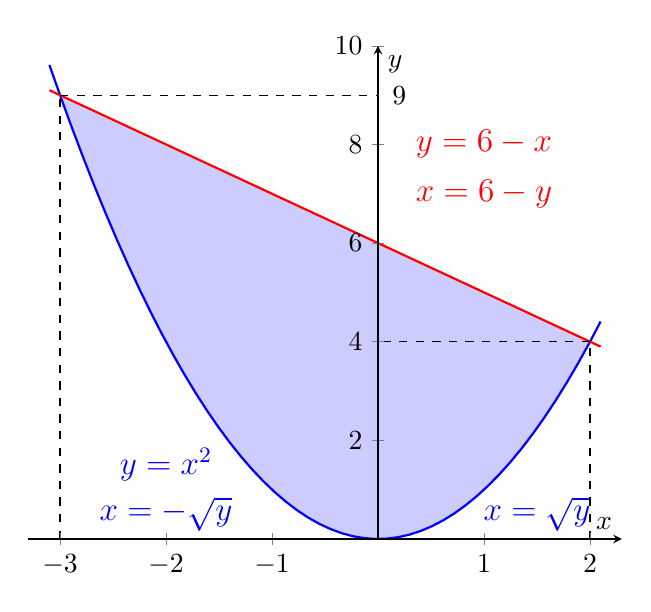
\begin{tikzpicture}
  \begin{axis}[
      axis lines=center,
      axis on top,
      xlabel={$x$},
      ylabel={$y$},
      xmin=-3.3, xmax=2.3,
      ymin=0, ymax=10,
      samples=50,
      clip=true,
      scale=1.1,
    ]
    
    \addplot [
        fill=blue!20,
        domain=-3:2,
        draw=none,
        name path=A,
    ] {x^2};
    
    \addplot [
        fill=white,
        domain=-3:2,
        draw=none,
        name path=B,
    ] {6-x};

    \addplot [
      blue!20,
      fill opacity=0.6,
    ] fill between[of=A and B];

    \addplot [
        thick,
        blue,
        domain=-3.1:2.1,
    ] {x^2};

    \addplot [
        thick,
        red,
        domain=-3.1:2.1,
        samples=200,
    ] {6-x};

    \node[blue] at (axis cs: -2, 1.5) {\large $y=x^2$};
    \node[blue] at (axis cs: -2, 0.5) {\large $x=-\sqrt y$};
    \node[blue] at (axis cs: 1.5, 0.5) {\large $x=\sqrt y$};
    \node[red] at (axis cs: 1, 8) {\large $y=6-x$};
    \node[red] at (axis cs: 1, 7) {\large $x=6-y$};
    
    \node at (axis cs: 0.2, 9) {$9$};

    \draw[black, dashed] (axis cs: 2,0) -- (axis cs: 2,4);
    \draw[black, dashed] (axis cs: -3,0) -- (axis cs: -3,9);
    \draw[black, dashed] (axis cs: -3,9) -- (axis cs: 0,9);
    \draw[black, dashed] (axis cs: 2,4) -- (axis cs: 0,4);
  \end{axis}
\end{tikzpicture}
\end{center}

\newpage

\begin{align*}\mathrm{I} &=\int_{-3}^2\int_{x^2}^{6-x}dy\,dx=\int_0^4\int_{-\sqrt y}^{\sqrt y}\,dx\,dy+\int_4^9\int_{-\sqrt y}^{6-y}\,dx\,dy\\\\&=\int_0^4\bigg[\sqrt y-\left(-\sqrt y\right)\bigg]\,dy+\int_4^9\bigg[(6-y)-(-\sqrt y)\bigg]\,dy\\\\&=2\int_0^4\sqrt y\,dy+\int_4^9(6-y+\sqrt y)\,dy=2\left[\frac23y^{3/2}\right]_0^4+\left[6y-\frac{y^2}2+\frac23y^{3/2}\right]_4^9\\\\&=\frac43\left[4^{3/2}-0^{3/2}\right]+\left[\left(6\cdot9-\frac{9^2}2+\frac23\cdot9^{3/2}\right)-\left(6\cdot4-\frac{4^2}2+\frac23\cdot4^{3/2}\right)\right]=\boxed{\frac{125}6}\end{align*}

\hfill

\noindent 3) We are interested in the upper half of the cardioid. Therefore, $0\leq\theta\leq\pi$.
\begin{center}
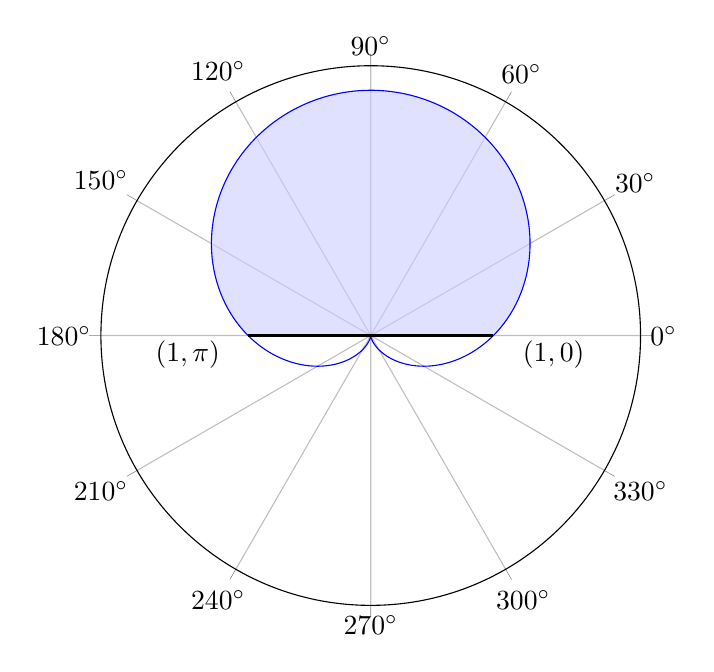
\begin{tikzpicture}
  \begin{polaraxis}[ytick=\empty, axis y line=none, xticklabel=$\pgfmathprintnumber{\tick}^\circ$,]
    \addplot [
      domain=0:pi,
      samples=100,
      draw=none,
      name path=A,
      data cs=polarrad,
    ] {1+sin(deg(x))};

    \addplot [
      name path=B,
    ] {0};

    \addplot [
      blue!20,
      fill opacity=0.6,
    ] fill between[of=A and B];

    \addplot [
      domain=0:2*pi,
      samples=300,
      blue,
      data cs=polarrad,
    ] {1+sin(deg(x))};
    
    \draw[black, thick] (axis cs: 0,-1) -- (axis cs: 0,1);
    \node at (axis cs: 6,-1.5) {$(1,\pi)$};
    \node at (axis cs: -6,1.5) {$(1,0)$};
  \end{polaraxis}
\end{tikzpicture}
\end{center}
\begin{align*}
\text{Area}&=\int_0^\pi\int_0^{1+\sin\theta}r\,dr\,d\theta=\frac12\int_0^\pi\left[(1+\sin\theta)^2-0^2\right]\,d\theta=\frac12\int_0^\pi\left(1+2\sin\theta+\sin^2\theta\right)\,d\theta\\\\&=\frac12\int_0^\pi\left(1+2\sin\theta+1-\cos^2\theta\right)\,d\theta=\frac12\int_0^\pi\left(1+2\sin\theta+\frac12-\frac{\cos(2\theta)}2\right)\,d\theta\\\\&=\frac12\left[\theta-2\cos\theta+\frac\theta2-\frac{\sin(2\theta)}4\right]_0^\pi\\\\&=\frac12\left[\left(\pi-2\cos\pi+\frac\pi2-\frac{\sin\left(2\pi\right)}4\right) - \left(0-2\cos0+0-\sin0\right)\right]=\boxed{\frac{3\pi}4+2}
\end{align*}

\newpage

\noindent 4)
\begin{center}
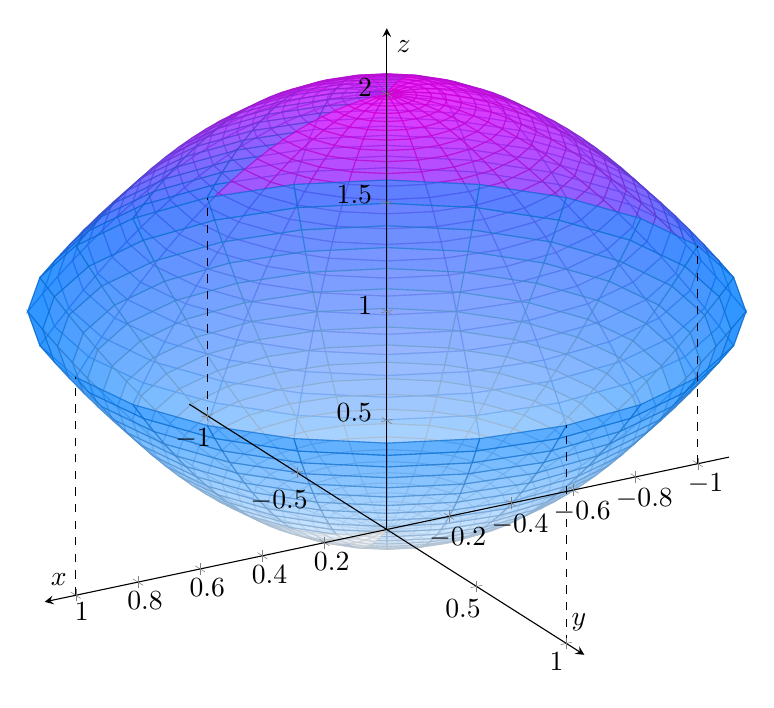
\begin{tikzpicture}
  \begin{axis}[
    view={150}{30},
    axis lines=center,
    axis on top,
    xlabel={$x$},
    ylabel={$y$},
    zlabel={$z$},
    xmin=-1.1, xmax=1.1,
    ymin=-1.1, ymax=1.1,
    zmin=0, zmax=2.3,
    colormap/cool,
    samples=25,
    domain=0:1,
    y domain=0:360,
    scale=2,
  ]

    \addplot3[
      surf,
      opacity=0.6,
      variable=\r,
      variable y=\t,
    ]
    ({r*cos(t)}, {r*sin(t)}, {2 - r^2});

    \addplot3[
      surf,
      opacity=0.6,
      variable=\r,
      variable y=\t,
    ]
    ({r*cos(t)}, {r*sin(t)}, {r^2});
    
    \draw[dashed] (axis cs:1,0,0)--(axis cs:1,0,1);
    \draw[dashed] (axis cs:-1,0,0)--(axis cs:-1,0,1);
    \draw[dashed] (axis cs:0,1,0)--(axis cs:0,1,1);
    \draw[dashed] (axis cs:0,-1,0)--(axis cs:0,-1,1);

  \end{axis}
\end{tikzpicture}
\end{center}
\begin{equation*}\mathrm{I}=\int_{-1}^1\int_{-\sqrt{1-x^2}}^{\sqrt{1-x^2}}\left[2-x^2-y^2-\left(x^2+y^2\right)\right]\,dy\,dx\end{equation*}

\hfill

\noindent This integral seems difficult. Use the transformation below to switch to polar coordinates.

\[
\begin{array}{c}
x^2+y^2=r^2\\
dA=dy\,dx =r\,dr\,d\theta
\end{array}\quad\rightarrow\quad
\begin{array}{c}
r^2\leq z\leq2-r^2\\
0\leq r\leq1\\
0\leq\theta\leq2\pi\\
\end{array}
\]

\begin{align*}\mathrm{I}&=\int_0^{2\pi}\int_0^1\left(2-2r^2\right)\,r\,dr\,d\theta=\int_0^{2\pi}\int_0^1\left(2r-2r^3\right)\,dr\,d\theta=\int_{0}^{2\pi}\left[r^2-\frac{r^4}2\right]_{r=0}^{r=1}\,d\theta\\\\&=\int_0^{2\pi}\frac12\,d\theta=\boxed\pi
\end{align*}

\hfill

\noindent 5) For the upper hemisphere, we have $z=\sqrt{4-x^2-y^2}$. The projection of the surface onto the $xy$-plane gives us the region $x^2+y^2\leq1$. Find the surface area.

\begin{align*}
\begin{array}{c}
\text{Surface}\\\text{area}
\end{array}&=\iint_D\sqrt{1+\left(\frac{\partial z}{\partial x}\right)^2+\left(\frac{\partial z}{\partial y}\right)^2}\,dA\\\\&=\int_{-1}^1\int_{-\sqrt{1-x^2}}^{\sqrt{1-x^2}}\sqrt{1+\left(\frac{x}{\sqrt{4-x^2-y^2}}\right)^2+\left(\frac{y}{\sqrt{4-x^2-y^2}}\right)^2}\,dy\,dx\\\\&=\int_{-1}^1\int_{-\sqrt{1-x^2}}^{\sqrt{1-x^2}}\sqrt{1+\frac{x^2+y^2}{4-x^2-y^2}}\,dy\,dx=\int_{-1}^1\int_{-\sqrt{1-x^2}}^{\sqrt{1-x^2}}\frac2{\sqrt{4-x^2-y^2}}\,dy\,dx\end{align*}

\newpage

\noindent From this point on, we can switch to polar coordinates using the transformation below.

\[
\begin{array}{c}
r^2=x^2+y^2\\
dA=r\,dr\,d\theta
\end{array}\quad\rightarrow\quad
\begin{array}{c}
\sqrt{4-x^2-y^2}=\sqrt{4-r^2}\\[0.3cm]
x^2+y^2\leq1\,\rightarrow\,r^2\leq1\implies0\leq r\leq1\\[0.3cm]
0\leq\theta\leq2\pi
\end{array}
\]

\begin{align*}
\begin{array}{c}
\text{Surface}\\\text{area}
\end{array}&=\int_{-1}^1\int_{-\sqrt{1-x^2}}^{\sqrt{1-x^2}}\frac2{\sqrt{4-x^2-y^2}}\,dy\,dx=\int_0^{2\pi}\int_0^1\frac2{\sqrt{4-r^2}}\cdot r\,dr\,d\theta\\\\&=\int_0^{2\pi}\left[-2\sqrt{4-r^2}\right]_{r=0}^{r=1}\,d\theta=\int_0^{2\pi}\left[-2\sqrt3-\left(-4\right)\right]\,d\theta=\boxed{4\pi\left(2-\sqrt3\right)}\end{align*}

\hfill

\noindent 6)

\hfill

\noindent (i)
\begin{center}
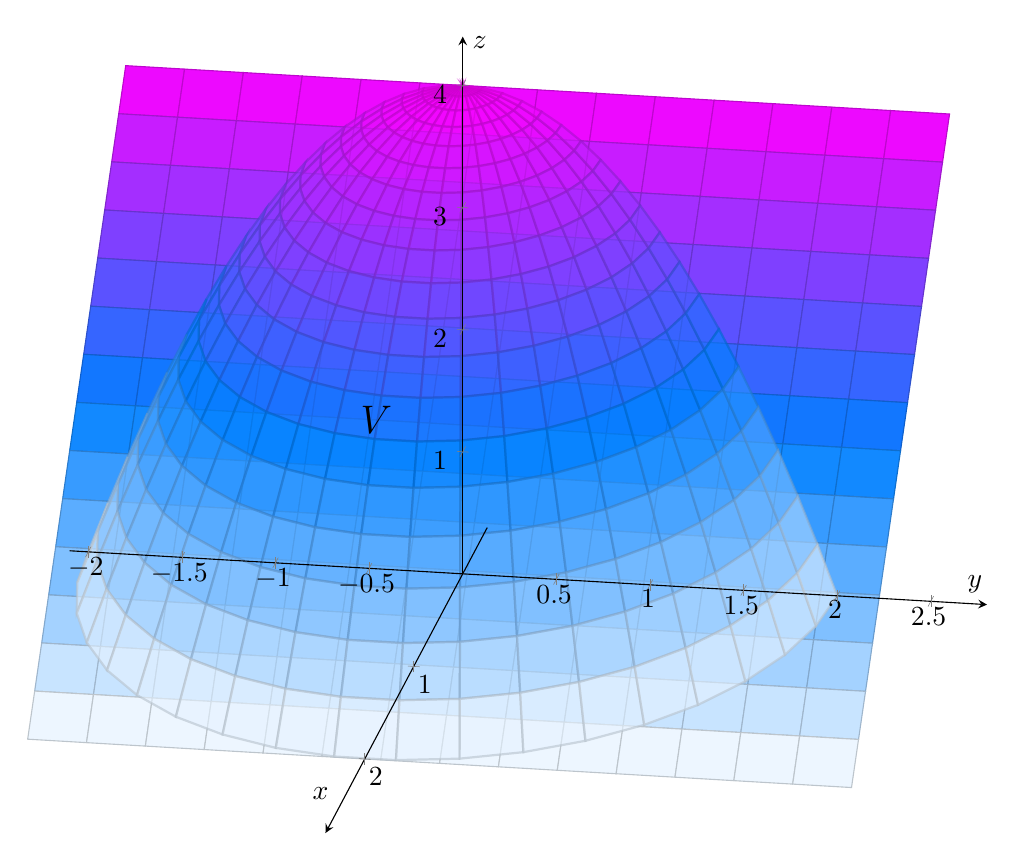
\begin{tikzpicture}
  \begin{axis}[
    view={100}{30},
    axis lines=center,
    axis on top,
    xlabel={$x$},
    ylabel={$y$},
    zlabel={$z$},
    xmin=-0.5, xmax=2.8,
    ymin=-2.1, ymax=2.8,
    zmin=0, zmax=4.4,
    domain=0:2,
    colormap/cool,
    scale=2,
  ]
    \addplot3[
      surf,
      y domain=-1.8:2.6,
      samples=15,
    ] {4 - 2*x};
    \addplot3[
      surf,
      opacity=0.6,
      variable=\r,
      variable y=\t,
      y domain=-90:90,
      samples=20,
      thick
    ]
    (
      {r*cos(t)},
      {r*sin(t)},
      {4 - (r*cos(t))^2 - (r*sin(t))^2}
    );
    \node at (1,-0.2,2) {\Large $V$};
  \end{axis}
\end{tikzpicture}
\end{center}

\hfill

\noindent (ii) Using cylindrical coordinates, we may find the volume.

\[
\begin{array}{c}
z=z\\
x=r\cos\theta\\
y=r\sin\theta\\
r^2=x^2+y^2\\
dV=r\,dz\,dr\,d\theta
\end{array}\quad\rightarrow\quad
\begin{array}{c}
z=4-x^2-y^2\implies z=4-r^2\\
z=4-2x\implies z=4-2r\cos\theta\\
4-2x=4-x^2-y^2 \implies r=2\cos\theta\\[0.3cm]
\displaystyle4-2r\cos\theta\leq z\leq 4-r^2,\quad0\leq r\leq2\cos\theta,\quad\frac{-\pi}2\leq\theta\leq\frac\pi2
\end{array}
\]

\newpage

\begin{align*}
V&=\int_{-\pi/2}^{\pi/2}\int_{0}^{2\cos\theta}\int_{4-2r\cos\theta}^{4-r^2}r\,dz\,dr\,d\theta=\int_{-\pi/2}^{\pi/2}\int_{0}^{2\cos\theta}\left[4-r^2-\left(4-2r\cos\theta\right)\right]\,r\,dr\,d\theta\\\\&=\int_{-\pi/2}^{\pi/2}\int_0^{2\cos\theta}(2r^2\cos\theta-r^3)\,dr\,d\theta=\int_{-\pi/2}^{\pi/2}\left[\frac{2r^3}3\cos\theta-\frac{r^4}4\right]_{r=0}^{r=2\cos\theta}\,d\theta\\\\&=\int_{-\pi/2}^{\pi/2}\left[\left(\frac{16}3\cos^4\theta-\frac{16\cos^4\theta}4\right) - 0\right]\,d\theta=\frac43\int_{-\pi/2}^{\pi/2}\cos^4\theta\,d\theta\\\\&=\frac43\int_{-\pi/2}^{\pi/2}\left(\frac{\cos(2\theta)+1}2\right)^2\,d\theta=\frac13\int_{-\pi/2}^{\pi/2}\left(\cos^2(2\theta)+2\cos(2\theta)+1\right)\,d\theta\\\\&=\frac13\int_{-\pi/2}^{\pi/2}\left[\left(\frac{\cos(4\theta)+1}2\right)+2\cos(2\theta)+1\right]\,d\theta=\frac13\left[\frac{\sin(4\theta)}8+\frac\theta2+\sin(2\theta)+\theta\right]_{-\pi/2}^{\pi/2}\\\\&=\frac13\left[\left(\frac{\sin(2\pi)}8+\frac\pi4+\sin\pi+\frac\pi2\right)-\left(\frac{\sin\left(-2\pi\right)}8-\frac\pi4+\sin(-\pi)-\frac\pi2\right)\right]=\boxed{\frac\pi2}
\end{align*}

\end{document}